\documentclass[11pt,3p]{elsarticle}


\usepackage{hyperref}
%\usepackage{lineno,hyperref}
\usepackage[toc,page]{appendix}
\usepackage{graphicx}
\usepackage{lscape}
\usepackage{multirow}
\usepackage{rotating}
\usepackage[table,xcdraw]{xcolor}
\usepackage{longtable}
\usepackage{threeparttable}
\usepackage{todonotes}
\usepackage{xcolor}
\usepackage{setspace}
\usepackage[font=normalsize,labelfont=bf]{caption}
\usepackage{bibentry}
%\usepackage{changes}
%\usepackage[final]{changes}
\usepackage{lineno}
%\setremarkmarkup{(#2)}
\interfootnotelinepenalty=10000
\renewcommand*{\today}{20.November.2018}
\newcommand{\RomanNumeralCaps}[1]{\MakeUppercase{\romannumeral #1}}
\newcommand{\MarieAnge}[1]{\todo[color=yellow!40]{#1}}
\newcommand{\Herve}[1]{\todo[color=blue!40]{#1}}
\newcommand{\Lei}[1]{\todo[color=purple!40]{#1}}
\renewcommand{\thefootnote}{}

%\modulolinenumbers[5]

\doublespacing

\journal{Renewable \& Sustainable Energy Reviews}

%% Numbered
%\bibliographystyle{model1-num-names}

%% Numbered without titles
%\bibliographystyle{model1a-num-names}

%% Harvard
%\bibliographystyle{model2-names.bst}\biboptions{authoryear}

%% Vancouver numbered
\usepackage{numcompress}\bibliographystyle{model3-num-names}

%% Vancouver name/year
%\usepackage{numcompress}\bibliographystyle{model4-names}\biboptions{authoryear}

%% APA style
%\bibliographystyle{model5-names}\biboptions{authoryear}

%% AMA style
%\usepackage{numcompress}\bibliographystyle{model6-num-names}

%% `Elsevier LaTeX' style
%\bibliographystyle{elsarticle-num}
%%%%%%%%%%%%%%%%%%%%%%%

\biboptions{sort&compress}

\begin{document}

\begin{frontmatter}

\title{Hydrogen supply chain network design: An optimization-oriented review}

\author[mymainaddress]{Lei Li\corref{mycorrespondingauthor}}
\cortext[mycorrespondingauthor]{Corresponding author}
\ead{lei.li1@utbm.fr}

\author[mymainaddress]{Herv\'{e} Manier}
\ead{herve.manier@utbm.fr}

\author[mymainaddress]{Marie-Ange Manier} 
\ead{marie-ange.manier@utbm.fr}

\address[mymainaddress]{Univ. Bourgogne Franche-Comt\'{e} FEMTO-ST Institute/CNRS,\\ UTBM, rue Thierry-Mieg, 90 010 Belfort Cedex, France}

\begin{abstract}

This study reviews the papers that pertain to the hydrogen supply chain network design (HSCND) models published in scientific journals. A few drawbacks (e.g., the treatment of uncertainty and feedstock problems) and missing aspects (e.g., the intertemporal integration planning) in the literature are identified, thus motivating the development of a comprehensive HSCND methodology. Key components of the hydrogen supply chain are presented; thereafter, the models are analyzed and classified based on their decisions, performance measures, uncertainties, solution methodologies, and other model features. Moreover, an effort was made to complete the critical pre-optimization preparation works, which are essential but have been overlooked in previous reviews. Finally, a list of potential problems for future research directions is recommended.

\end{abstract}

\begin{keyword}
Hydrogen, Supply chain, Network design, Optimization models
\end{keyword}

\footnotetext{\textit{Abbreviations:} BG, biomass gasification; CCS, carbon capture and storage; CG, coal gasification; GH2, gaseous hydrogen; DP, dynamic programming; FCEV, fuel cell electric vehicle; GIS, geographic information system; HSC, hydrogen supply chain; HSCND, hydrogen supply chain network design; IEA, International Energy Agency; LCA, life cycle assessment; LH2, liquid hydrogen; LP, linear programming; MARKAL, MARKet and ALlocation; MILP, mixed-integer linear programming; SC, supply chain; SCM, supply chain management; SCND, supply chain network design; SMR, steam methane reforming; T\&D, transportation and distribution; TIMES, The Integrated MARKAL-EFOM System.}

\end{frontmatter}

%\linenumbers

\section{Introduction}
\label{sec:intro}

With the implementation of the Paris Agreement on November 4, 2016, expectations are growing for hydrogen energy as a dynamic vector. Because the 2$^\circ$C warming scenario has been established to attain a carbon emission trajectory that limits the concentration of greenhouse gases in the atmosphere, the ability to reduce emissions without jeopardizing economic growth has been the objective pursued by governments and climate change campaigners alike, especially in emerging markets. It is assumed that the utilization of hydrogen not only can enhance the sustainability and reliability of the energy system, but also perform a significant function in the system's flexibility. The International Energy Agency (IEA) \citep{iea2015technology} noted that the use of hydrogen could link different energy sectors and energy transportation and distribution (T\&D) networks; thus, it could increase the operational flexibility of future low-carbon energy systems. Today's energy system is heavily dependent on fossil fuels; moreover, apart from co-generation, few connections exist among the different T\&D systems. In a future system, hydrogen could perform a pivotal function by linking various layers of infrastructures in a low-carbon energy system.

Hydrogen technologies and products have significantly progressed over the years and are currently being established in the market. Generally, the insufficiency of the present infrastructure is considered one of the barriers to boost the hydrogen economy. Accordingly, large-scale infrastructure investment schemes based on the development of new strategies should be conducted. Moreover, the industry has endeavored to promote the growth of hydrogen consumption. In January 2017, 13 leading companies in energy, transport, and industry launched a global initiative---the ``Hydrogen Council''---to express a unified vision and long-term goal for the used of hydrogen to foster energy transition \citep{Hydrogen}. In its new roadmap published in November 2017 \citep{HydrogenCouncil2017}, the Hydrogen Council indicated that by 2050, hydrogen could satisfy 18\% of the world's total energy demands and reduce CO$_{2}$ emissions in various sectors, such as residential, transport, and industry, by 40-60\%. Moreover, policymakers and researchers continue to investigate the applicability and problems of shifting from an unsustainable carbon-based economy to a sustainable hydrogen-based economy. In general, one of the foremost concerns is the formulation of a strategy that could realize the aforementioned vision; the answers to the ``4w questions'' summarizes this strategy. That is, the temporal and spatial decisions to build hydrogen infrastructures---when, where, at what sizes and with which technologies \citep{lin2008least}.

\begin{figure}[!htbp]
\centering
\includegraphics[width=1\textwidth]{FIG_1}
\caption{\label{fig:NetworkRepresentHSC}Hydrogen supply chain network (HSCN) in the transportation sector}
\end{figure}

The supply chain network design (SCND), also referred to as the strategic supply chain planning is one of the most crucial planning problems in the supply chain management (SCM) \citep{govindan2017supply}. The concept of the hydrogen supply chain network design (HSCND) is adopted for investigating the deployment of hydrogen infrastructures. The hydrogen supply chain network (HSCN) in the transportation sector is depicted in Fig. \ref{fig:NetworkRepresentHSC}. It begins at the feedstock and ends at the selling of hydrogen at refueling stations. There are multiple choices available in each section. For instance, water (with electricity), biomass, and coal could be utilized as feedstock for the production process of electrolysis, biomass gasification (BG), and coal gasification (CG), respectively. Thereafter, the hydrogen produced can be transported to terminals via trucks, trains, or pipelines. Various storage approaches can be selected in terminals based on the physical form of hydrogen. There are two primary types of refueling stations---standard and on-site, which are further explained in Section \ref{sec:system}. Because of the inherent characteristics of a supply chain, each part is interconnected rather than isolated. In all types of renewable and sustainable energy, the development of a competitive market requires complex design, planning, and optimization methods. These has been observed in several optimization methods, which have been applied to the field of renewable and sustainable energy \citep{banos2011optimization,de2014methods}. The complexity of the problem in the HSCND depends on the modeling of the interactions that exist between the different parts of the HSCN. Specifically, the production technologies are dependent on the regionally unique characteristics of feedstocks; note that storage and transportation modes have strong relationships with the physical form of hydrogen. Moreover, the locations and technologies of refueling stations are significantly affected by the structure of the hydrogen supply network. The optimization-based approach has been particularly influential in contributing insights into these technological and spatial interactions. After a two-decade development, an increasing number of research studies on the HSCND are now available to provide an understanding of a future HSCN in the transportation sector. This study aims to review the papers pertaining to the HSCND models published in scientific journals. To determine the research opportunities and future directions, the gaps existing in the present literature are clearly explained as well.

The present paper is organized as follows. Three previous review papers on the HSCND are discussed in Section \ref{sec:motivation}. Section \ref{sec:review} describes the methodology adopted for the collection of research papers. A classification of the optimization-based studies of HSCND is performed; thereafter, papers for further analysis are selected. In Section \ref{sec:system}, a detailed system analysis is presented. Modeling approaches and solution methods are explained in Section \ref{sec:model}. Section \ref{sec:pre-optimi} is a special section that reports on the key pre-optimization preparation works. Particular emphasis is given to data collection and hydrogen demand estimation. In the final section, a list of potential problems for future research directions is recommended.

\section{Research motivation}
\label{sec:motivation}

Limited reviews are available on the HSCND in the literature and have not covered all aspects of the problem it involves. This present review aims to complete this insufficiency. In this section, three previous review papers are analyzed. \citet{dagdougui2012models} firstly conducted a system analysis of the HSCN, which includes feedstock and production, transportation, and end users. Afterwards,  \citet{dagdougui2012models} discussed several hydrogen economy roadmaps that are deployed by different countries as well as conceptualized scenarios, which can be considered as systematic tools to support the HSCND. \citet{dagdougui2012models} classified the approaches for the HSCND into three categories: optimization methods, geographical information system (GIS), and assessment plans toward the transition to a hydrogen infrastructure. The HSCND models in literature are studied, but detailed classification and analysis are not performed from the aspect of decisions, performance measures, and uncertainty problems. \citet{agnolucci2013designing} examined the HSCND studies across spatial scales: national scale studies using energy system models, regional-scale studies that optimize spatially disaggregated hydrogen infrastructure, and local-scale studies that optimize the siting of refueling stations. For the two latter types of studies, \citet{agnolucci2013designing} critically assessed the assumptions made regarding hydrogen demand, which they supposed as a critical exogenous input into these studies. The unusual perspective (across different spatial scales) enables the authors to conduct a more in-depth analysis and therefore provide reasonable research directions. Similar to the review performed by \citet{dagdougui2012models}, detailed classification and analysis through decisions, performance measures, and uncertainty problems are neglected. Moreover, in this review, system analysis is not included. \citet{maryam2017review} reviewed the modeling approaches used in the HSCND for the UK. A classification of these approaches is accomplished based on optimization approaches, GIS, transition models, and system dynamic approaches. Although the system analysis is provided, it is not comprehensive. Performance measures, such as the minimization of costs and the reduction of environmental impacts, are analyzed. However, decision levels, decision variables, and uncertainty problems are not discussed.

To our best knowledge, no comprehensive review of the optimization models for the HSCND problem has yet been performed. Therefore, this study aims to analyze and classify the entities and technologies (hydrogen production, transportation, etc.) studied in each model to identify which combinations have been and have not been covered. A detailed classification from the aspect of decisions, performance measures, and uncertainty problems to specify the contributions as well as research gaps is also provided. Moreover, some critical factors that have been neglected in previous reviews, such as solution methods and key pre-optimization preparation works are considered in this research to provide a broad view for the readers.

\section{Classification of review papers}
\label{sec:review}

\subsection{Search for literature}
\label{sec:searchliter}

A thorough search for related research over the last decade is implemented to produce a synthesis of the peer-reviewed literature. Papers published in international peer-reviewed journals from the main electronic bibliographical sources (Scopus, Web of Science) are searched by entering keywords, such as hydrogen, supply chain, infrastructure, optimization, and network design in the titles or the topics covered. In all, 71 papers are collected. Figure \ref{fig:DistributionPapers} displays the yearly distribution of these papers, which can be found in 16 distinct journals. Most of these have been published in the \textit{International Journal of Hydrogen Energy}; a few could be found in journals of operations research. The latter is certainly surprising because the papers propose optimization models based on operations research methods. These papers are classified according to the following: model type, research object, spatial scale, and whether a full description of the mathematical formulations is included. The individual characteristics of each paper are listed in Tables \ref{tab:CharaHSCND1} and \ref{tab:CharaHSCND2}. It can be found that linear programming and mixed-integer linear programming (LP/MILP) models are mostly used, and only three studies adopted the dynamic programming (DP) models. A large portion of the studies tackled the multi-echelon problem. This is because one of the significant advantages of the LP/MILP model is accounting for the complex interactions among different echelons. In terms of the spatial scale, the national and regional planning problems received more attention than international and urban problems. 

\begin{figure}[!htbp]
\centering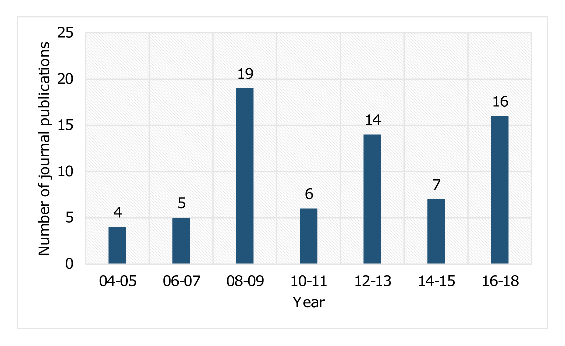
\includegraphics[width=0.6\textwidth]{FIG_2}
\caption{\label{fig:DistributionPapers}Distribution of papers (up to June 2018)}
\end{figure}

\begin{table}[!htbp]
\caption{Individual characteristics of optimization-based models for HSCND (Part 1)}
\label{tab:CharaHSCND1}
\resizebox{\textwidth}{!}{
\begin{tabular}{lccccccccccccc}
\hline
 & \multicolumn{3}{c}{Model type} & \multicolumn{4}{c}{Research object} & \multicolumn{4}{c}{Spatial scale} & \multicolumn{2}{c}{Full description} \\
 & DP & \multicolumn{2}{c}{LP / MILP} & Multi-E & \multicolumn{3}{c}{Mono-E} & I & N & R & U & Yes & No \\
 &  & ESM & GEM &  & P & T & RS &  &  &  &  &  &  \\ \hline
\citet{agnolucci2013importance} &  &  & $\bullet$ & $\bullet$ &  &  &  &  & $\bullet$ &  &  & $\bullet$ &  \\
\citet{almansoori2016design} &  &  & $\bullet$ & $\bullet$ &  &  &  &  & $\bullet$ &  &  & $\bullet$ &  \\
\citet{almansoori2006design} &  &  & $\bullet$ & $\bullet$ &  &  &  &  & $\bullet$ &  &  & $\bullet$ &  \\
\citet{almansoori2009design} &  &  & $\bullet$ & $\bullet$ &  &  &  &  & $\bullet$ &  &  & $\bullet$ &  \\
\citet{almansoori2012design} &  &  & $\bullet$ & $\bullet$ &  &  &  &  & $\bullet$ &  &  & $\bullet$ &  \\
\citet{almaraz2013assessment} &  &  & $\bullet$ & $\bullet$ &  &  &  &  & $\bullet$ &  &  & $\bullet$ &  \\
\citet{almaraz2014hydrogen} &  &  & $\bullet$ & $\bullet$ &  &  &  &  &  & $\bullet$ &  & $\bullet$ &  \\
\citet{almaraz2015deployment} &  &  & $\bullet$ & $\bullet$ &  &  &  &  & $\bullet$ &  &  & $\bullet$ &  \\
\citet{amoo2014integrated} &  & $\bullet$ &  & $\bullet$ &  &  &  &  & $\bullet$ &  &  &  & $\bullet$ \\
\citet{andre2013design} &  &  & $\bullet$ &  &  & $\bullet$ &  &  & $\bullet$ &  &  & $\bullet$ &  \\
\citet{andre2014time} &  &  & $\bullet$ &  &  & $\bullet$ &  &  & $\bullet$ &  &  &  & $\bullet$ \\
\citet{ball2007integration} &  &  & $\bullet$ & $\bullet$ &  &  &  &  & $\bullet$ &  &  &  & $\bullet$ \\
\citet{balta2013spatial} &  & $\bullet$ & $\bullet$ & $\bullet$ &  &  &  &  & $\bullet$ &  &  &  & $\bullet$ \\
\citet{bersani2009network} &  &  & $\bullet$ &  &  &  & $\bullet$ &  &  & $\bullet$ &  & $\bullet$ &  \\
\citet{bique2018balancing} &  &  & $\bullet$ & $\bullet$ &  &  &  &  & $\bullet$ &  &  &  & $\bullet$ \\
\citet{bique2018outlook} &  &  & $\bullet$ & $\bullet$ &  &  &  &  & $\bullet$ &  &  & $\bullet$ &  \\
\citet{brey2006designing} &  &  & $\bullet$ & $\bullet$ &  &  &  &  & $\bullet$ &  &  & $\bullet$ &  \\
\citet{brey2012using} &  &  & $\bullet$ &  &  &  & $\bullet$ &  &  & $\bullet$ &  &  & $\bullet$ \\
\citet{cho2016optimization} &  &  & $\bullet$ & $\bullet$ &  &  &  &  & $\bullet$ &  &  & $\bullet$ &  \\
\citet{contaldi2008hydrogen} &  & $\bullet$ &  & $\bullet$ &  &  &  &  & $\bullet$ &  &  &  & $\bullet$ \\
\citet{contreras2009market} &  & $\bullet$ &  & $\bullet$ &  &  &  &  &  & $\bullet$ &  &  & $\bullet$ \\
\citet{dagdougui2012modelling} &  &  & $\bullet$ & $\bullet$ &  &  &  &  &  & $\bullet$ &  & $\bullet$ &  \\
\citet{dayhim2014planning} &  &  & $\bullet$ & $\bullet$ &  &  &  &  &  & $\bullet$ &  & $\bullet$ &  \\
\citet{endo2007market} &  & $\bullet$ &  & $\bullet$ &  &  &  &  & $\bullet$ &  &  &  & $\bullet$ \\
\citet{gim2012transportation} &  &  & $\bullet$ &  &  & $\bullet$ &  &  & $\bullet$ &  &  & $\bullet$ &  \\
\citet{guillen2010bi} &  &  & $\bullet$ & $\bullet$ &  &  &  &  & $\bullet$ &  &  & $\bullet$ &  \\
\citet{gul2009energy} &  & $\bullet$ &  & $\bullet$ &  &  &  & $\bullet$ &  &  &  &  & $\bullet$ \\
\citet{hajimiragha2009hydrogen} &  &  & $\bullet$ &  & $\bullet$ &  &  &  &  & $\bullet$ &  & $\bullet$ &  \\
\citet{han2012modeling} &  &  & $\bullet$ & $\bullet$ &  &  &  &  & $\bullet$ &  &  & $\bullet$ &  \\
\citet{han2013multi} &  &  & $\bullet$ & $\bullet$ &  &  &  &  & $\bullet$ &  &  & $\bullet$ &  \\
\citet{he2017hydrogen} &  &  & $\bullet$ &  &  &  & $\bullet$ &  &  & $\bullet$ &  & $\bullet$ &  \\
\citet{hugo2005hydrogen} &  &  & $\bullet$ & $\bullet$ &  &  &  &  &  &  &  &  & $\bullet$ \\
\citet{hwangbo2017mathematical} &  &  & $\bullet$ & $\bullet$ &  &  &  &  & $\bullet$ &  &  & $\bullet$ &  \\
\citet{ingason2008optimizing} &  &  & $\bullet$ &  & $\bullet$ &  &  &  & $\bullet$ &  &  & $\bullet$ &  \\
\citet{johnson2012spatially} &  &  & $\bullet$ & $\bullet$ &  &  &  &  &  & $\bullet$ &  & $\bullet$ &  \\
\citet{johnson2005optimal} &  &  & $\bullet$ & $\bullet$ &  &  &  &  &  & $\bullet$ &  &  & $\bullet$ \\ \hline
\end{tabular}
}
\begin{tablenotes}
\small
\item ESM, energy system model; GEM, geographically explicit model; Multi-E, multi-echelon; Mono-E, mono-echelon; P, production; T, transportation; RS, refueling station; I, international; N, national; R, regional; U, urban.
\end{tablenotes}
\end{table}

\begin{table}[!htbp]
\caption{Individual characteristics of optimization-based models for HSCND (Part 2)}
\label{tab:CharaHSCND2}
\resizebox{\textwidth}{!}{
\begin{tabular}{lccccccccccccc}
\hline
 & \multicolumn{3}{c}{Model type} & \multicolumn{4}{c}{Research object} & \multicolumn{4}{c}{Spatial scale} & \multicolumn{2}{c}{Full description} \\
 & DP & \multicolumn{2}{c}{LP / MILP} & Multi-E & \multicolumn{3}{c}{Mono-E} & I & N & R & U & Yes & No \\
 &  & ESM & GEM &  & P & T & RS &  &  &  &  &  &  \\ \hline
\citet{kamarudin2009synthesis} &  &  & $\bullet$ & $\bullet$ &  &  &  &  & $\bullet$ &  &  & $\bullet$ &  \\
\citet{kim2008strategic} &  &  & $\bullet$ & $\bullet$ &  &  &  &  & $\bullet$ &  &  & $\bullet$ &  \\
\citet{kim2008optimization} &  &  & $\bullet$ & $\bullet$ &  &  &  &  & $\bullet$ &  &  & $\bullet$ &  \\
\citet{konda2011optimal} &  &  & $\bullet$ & $\bullet$ &  &  &  &  & $\bullet$ &  &  & $\bullet$ &  \\
\citet{konda2012dutch} &  &  & $\bullet$ & $\bullet$ &  &  &  &  & $\bullet$ &  &  &  & $\bullet$ \\
\citet{krishnan2014planning} &  &  & $\bullet$ & $\bullet$ &  &  &  &  & $\bullet$ &  &  &  & $\bullet$ \\
\citet{krzyzanowski2008supporting} &  & $\bullet$ &  & $\bullet$ &  &  &  & $\bullet$ &  &  &  &  & $\bullet$ \\
\citet{kuby2009optimization} &  &  & $\bullet$ &  &  &  & $\bullet$ &  &  & $\bullet$ &  & $\bullet$ &  \\
\citet{lahnaoui2018optimizing} &  &  & $\bullet$ &  &  & $\bullet$ &  &  &  & $\bullet$ &  & $\bullet$ &  \\
\citet{li2008hydrogen} &  &  & $\bullet$ & $\bullet$ &  &  &  &  & $\bullet$ &  &  &  & $\bullet$ \\
\citet{lin2008fuel} &  &  & $\bullet$ &  &  &  & $\bullet$ &  &  & $\bullet$ &  & $\bullet$ &  \\
\citet{lin2006hydrogen} & $\bullet$ &  &  & $\bullet$ &  &  &  &  &  &  & $\bullet$ & $\bullet$ &  \\
\citet{lin2008least} & $\bullet$ &  &  & $\bullet$ &  &  &  &  &  & $\bullet$ &  & $\bullet$ &  \\
\citet{kim2016optimization} &  &  & $\bullet$ & $\bullet$ &  &  &  &  & $\bullet$ &  &  & $\bullet$ &  \\
\citet{kim2017integrated} &  &  & $\bullet$ & $\bullet$ &  &  &  &  &  & $\bullet$ &  & $\bullet$ &  \\
\citet{moreno2017towards} &  &  & $\bullet$ & $\bullet$ &  &  &  &  & $\bullet$ &  &  & $\bullet$ &  \\
\citet{nunes2015design} &  &  & $\bullet$ & $\bullet$ &  &  &  &  & $\bullet$ &  &  & $\bullet$ &  \\
\citet{ogumerem2017multi} &  &  & $\bullet$ & $\bullet$ &  &  &  &  &  & $\bullet$ &  & $\bullet$ &  \\
\citet{parker2010waste} &  &  & $\bullet$ & $\bullet$ &  &  &  &  &  & $\bullet$ &  & $\bullet$ &  \\
\citet{qadrdan2008model} & $\bullet$ &  &  & $\bullet$ &  &  &  &  & $\bullet$ &  &  & $\bullet$ &  \\
\citet{rits2004evaluating} &  & $\bullet$ &  & $\bullet$ &  &  &  &  & $\bullet$ &  &  &  & $\bullet$ \\
\citet{rosenberg2010market} &  & $\bullet$ & $\bullet$ & $\bullet$ &  &  &  &  & $\bullet$ &  &  &  & $\bullet$ \\
\citet{sabio2010strategic} &  &  & $\bullet$ & $\bullet$ &  &  &  &  & $\bullet$ &  &  & $\bullet$ &  \\
\citet{sabio2012holistic} &  &  & $\bullet$ & $\bullet$ &  &  &  &  & $\bullet$ &  &  & $\bullet$ &  \\
\citet{samsatli2016optimal} &  &  & $\bullet$ & $\bullet$ &  &  &  &  & $\bullet$ &  &  & $\bullet$ &  \\
\citet{sgobbi2016far} &  & $\bullet$ &  & $\bullet$ &  &  &  & $\bullet$ &  &  &  &  & $\bullet$ \\
\citet{stephens2010systematic} &  &  & $\bullet$ &  &  &  & $\bullet$ &  &  &  & $\bullet$ &  & $\bullet$ \\
\citet{strachan2009soft} &  & $\bullet$ &  & $\bullet$ &  &  &  &  & $\bullet$ &  &  &  & $\bullet$ \\
\citet{sun2017hydrogen} &  &  & $\bullet$ &  &  &  & $\bullet$ &  &  & $\bullet$ &  & $\bullet$ &  \\
\citet{tseng2005hydrogen} &  & $\bullet$ &  & $\bullet$ &  &  &  &  & $\bullet$ &  &  &  & $\bullet$ \\
\citet{winskel2009decarbonising} &  & $\bullet$ &  & $\bullet$ &  &  &  &  & $\bullet$ &  &  &  & $\bullet$ \\
\citet{won2017design} &  &  & $\bullet$ & $\bullet$ &  &  &  &  &  & $\bullet$ &  & $\bullet$ &  \\
\citet{woo2016optimization} &  &  & $\bullet$ & $\bullet$ &  &  &  &  &  & $\bullet$ &  & $\bullet$ &  \\
\citet{yang2013renewable} &  & $\bullet$ &  & $\bullet$ &  &  &  &  &  & $\bullet$ &  &  & $\bullet$ \\
\citet{yeh2008optimizing} &  & $\bullet$ &  & $\bullet$ &  &  &  &  & $\bullet$ &  &  &  & $\bullet$ \\ \hline
\end{tabular}%
}
\begin{tablenotes}
\small
\item ESM, energy system model; GEM, geographically explicit model; Multi-E, multi-echelon; Mono-E, mono-echelon; P, production; T, transportation; RS, refueling station; I, international; N, national; R, regional; U, urban.
\end{tablenotes}
\end{table}

According to \citet{agnolucci2013designing}, these optimization-based HSCND models could further be grouped into three main categories (Table \ref{tab:ThreeTypesModels}). 

\begin{table}[!htbp]
\centering
\caption{Three main types of HSCND models}
\label{tab:ThreeTypesModels}
\begin{tabular}{lcc}
\hline
 & Research object & Spatial scale \\ \hline
Energy system optimization models & Entire HSCN & International/National/Regional \\
Geographically explicit optimization models & Entire HSCN & National/Regional \\
Refueling station locating models & Part of HSCN & Urban \\ \hline
\end{tabular}
\end{table}

\textit{Energy system optimization models.} These models use the LP/MILP to identify the energy system that meets energy service demands at minimal cost. They can be implemented at different spatial scales, i.e., international, national, or regional. Energy system models typically include a detailed HSCND with the representation of various feedstocks, hydrogen production technologies, and transportation modes. Hydrogen end-use technologies compete with others (such as battery electric vehicles) to meet energy service demands (such as demands for car transport); thus, hydrogen demand and supply are both endogenously optimized \citep{agnolucci2013designing}. The MARKAL/TIMES family is the most represented among the energy system models. MARKAL is a demand-driven multi-period LP model of energy supply and demand \citep{Rath1982energy} (TIMES is a successor of MARKAL). It was developed by the IEA's Energy Technology Systems Analysis Program in the 1980s. The MARKAL/TIMES model has been adopted to evaluate the role of hydrogen within an energy system in China \citep{rits2004evaluating}, the US \citep{tseng2005hydrogen,yeh2008optimizing}, the UK \citep{strachan2009soft,winskel2009decarbonising}, Italy \citep{contaldi2008hydrogen}, Spain \citep{contreras2009market}, Norway \citep{rosenberg2010market}, Japan \citep{endo2007market}, and at international scales \citep{gul2009energy}.

\textit{Geographically explicit optimization models.} These models also consider the entire HSCN and run at a national or a regional scale. Unlike energy system models, geographically explicit models focus on the deployment of hydrogen infrastructures. Binary and integer decision variables are employed to cope with the location of facilities, sizing decisions, selection of suitable production technology, and selection of transportation modes among facilities. Because product flows along the supply chain are modeled by continuous constraints, these models are often mixed-integer formulations \citep{eskandarpour2015sustainable}. For instance, \citet{almansoori2006design} established a steady-state ``snapshot'' model that integrates multiple components, such as production, storage, and transportation within a single framework; Great Britain was selected as case study. Subsequently, \citet{almansoori2009design} extended their study by considering the availability of feedstocks and their logistics, as well as the variation of hydrogen demand over a long-term planning horizon leading to a phased infrastructure development. \citet{samsatli2016optimal} developed a general spatio-temporal model that determines the optimal HSCN structure and its operation; the long-term planning horizon and short-term dynamics are simultaneously considered. The spatial distribution and temporal variability of hydrogen demands and wind availability are considered in detail in the model. The objective is the minimization of the total network cost, subject to satisfying all the demands of the domestic transport sector in Great Britain. 

\textit{Refueling station-locating models.} The construction of refueling infrastructures is one of the most formidable barriers to the transition to a hydrogen-based road transportation system \citep{national2004hydrogen}. Given the high cost of building new refueling stations, it is essential to coordinate the locations of initial stations in a network to facilitate maximum consumer utilization \citep{kuby2009optimization}. Based on the classical facility location models, a number of new models have been developed to optimize a network of hydrogen refueling stations in a relatively small geographical space, generally a big city, or sometimes, a state (region). For example, \citet{lin2008fuel} developed a locating method where station siting is treated as a ``fuel-travel-back'' problem, and the only required input is the distribution of vehicle miles traveled. The model was applied to derive an optimal station roll-out scheme for Southern California. \citet{kuby2005flow} introduced the ``Flow-Refueling Location Model'' that locates alternative fuel stations to refuel a maximum volume of vehicle flows. The model was used to investigate strategies for initial hydrogen refueling infrastructure deployment in Florida \citep{kuby2009optimization}. \citet{bersani2009network} presented a model for planning a refueling station network of a given company within a competitive framework; the model was tested in a specific territory in northern Italy. \citet{he2017hydrogen} created a hydrogen refueling station-siting optimization model for hydrogen energy expressway construction based on the energy life cycle cost analysis of hydrogen. \citet{sun2017hydrogen} determined optimal station construction locations on condition of multi-source hydrogen supply. A particle swarm optimization algorithm was created for the station location problem along the Shanghai-Nanjing Expressway in eastern China. 

\subsection{Selection of papers for further analysis}

The papers are filtered for a 
detailed investigation as described in the following sections. Based on the purpose of this work, the following criteria are established: (i) the models in the papers must consider the entire HSCN as the research object; (ii) they must include definitions of objective functions, decision variables, and constraints; (iii) explicit description of mathematical formulation must be offered. Based on the first criterion, some articles that only partially consider the HSCN are excluded. This is the case for studies that deal with refueling station-siting problems and those that focus on the problem of hydrogen production and transportation \citep{andre2013design,lahnaoui2018optimizing}. The second and third criteria enable the authors to filter the studies that adopt the energy system model and several other papers that provide limited information on the model used in the analysis; examples of these are the works of \citet{ball2007integration}, \citet{bique2018balancing}, \citet{hugo2005hydrogen} and \citet{li2008hydrogen}. Finally, 32 papers are identified and denoted as \textit{reference papers}. HistCite \citep{garfield2004histcite} is used to examine the citational relationships among the reference papers. It is found that the work of \citet{almansoori2006design} is the seminal paper in this branch of the literature. This paper has been a source of inspiration for other reference papers, which have attempted to improve it through multiple modifications \citep{agnolucci2013designing}. As summarized in Table \ref{tab:Modifications}, these modifications have been classified into four categories. More detailed model characteristics are discussed in following sections. In this table, the modifications conducted in each reference paper in each year are briefly described to reveal the strong connections among the reference papers. This confirmed the paper selection and motivated the authors to investigate the role of the optimization-based approach in the HSCND by examining the characteristics of this \textit{model group}.

\begin{table}[!htbp]
\centering
\caption{Four types of modifications of Ref. \citep{almansoori2006design} performed in reference papers}
\label{tab:Modifications}
\begin{tabular}{ccccc}
\hline
Year & \multicolumn{1}{l}{Implementing a multi-} & \multicolumn{1}{l}{Implementing a multi-} & \multicolumn{1}{l}{Introducing} & \multicolumn{1}{l}{Integration with} \\
 & \multicolumn{1}{l}{objective optimization} & \multicolumn{1}{l}{period optimization} & \multicolumn{1}{l}{uncertainty} & \multicolumn{1}{l}{other supply chains} \\ \hline
2008 & \citep{kim2008strategic} &  &  &  \\
2009 &  &  & \citep{kim2008optimization} &  \\
2010 & \citep{guillen2010bi} & \citep{almansoori2009design} & \citep{sabio2010strategic} &  \\
2011 &  & \citep{konda2011optimal} &  &  \\
2012 & \citep{sabio2012holistic} &  & \citep{almansoori2012design} &  \\
2013 & \citep{han2013multi,almaraz2013assessment} &  &  & \citep{agnolucci2013importance} \\
2014 & \citep{almaraz2014hydrogen} & \citep{almaraz2014hydrogen} & \citep{dayhim2014planning} &  \\
2015 & \citep{almaraz2015deployment} & \citep{almaraz2015deployment} & \citep{nunes2015design} &  \\
2016 &  & \citep{moreno2017towards} &  & \citep{ball2007integration,kim2016optimization,woo2016optimization,cho2016optimization} \\
2017 & \citep{ogumerem2017multi} & \citep{ogumerem2017multi} &  & \citep{won2017design,hwangbo2017mathematical} \\ \hline
\end{tabular}
\end{table}

All the mathematical models built in the studies reported in the reference papers are MILP-based and focus on the deployment of hydrogen in the transport sector. The key modeling features (i.e., system analysis, modeling approaches, and solution methods) are analyzed in the following two sections.

\section{System analysis}
\label{sec:system}

\citet{diwekar2008introduction} concludes that optimization involves several steps; the first step is to understand the system. The robustness of an HSCND model is based on the degree of understanding the real system. The descriptive superstructure of an HSCN in the transportation sector is illustrated in Fig. \ref{fig:Superstructure}. In this section, each key component of the system is examined to identify the entities and technologies that have been considered in the HSCND models. The aspects that require more attention are also identified.

\begin{figure}[!htbp]
\centering\includegraphics[width=0.9\textwidth]{FIG_3}
\caption{\label{fig:Superstructure}Superstructure of HSCN in the transportation sector (adapted from \citet{moreno2017towards})}
\end{figure}

\subsection{Feedstock}

Hydrogen is not an energy source; it is an energy carrier, which produced by various feedstocks \citep{ren2013sustainability}. Natural gas, coal, biomass, and water (with electricity from the local power grid) are the feedstocks found in most of the research projects \citep{agnolucci2013importance,almansoori2012design,kim2008optimization,kim2008strategic,nunes2015design}. Because concepts, such as low-carbon electrolytic hydrogen and CO$_{2}$-free HSCN has gained increasing attention in the post-Paris Agreement era, renewable sources have become more popular \citep{abbasi2011renewable,chattanathan2012review}. Figure \ref{fig:SourceElectricity} shows that in addition to the traditional source (power grid), some other sources of electricity have also been considered; several models include renewable energy-based electricity. For instance, \citet{kim2017integrated} designed a wind-based hydrogen system. \citet{won2017design}, and \citet{kim2016optimization} focused on the renewable energy source-based hydrogen supply system, in which the biomass, solar electricity, and wind power were selected. \citet{almaraz2014hydrogen} included four sources of electricity: solar, wind, hydro-power, and nuclear. Regarding the nuclear source, a more recent paper \citep{cany2017adapting} discussed the possibility of adopting the French nuclear fleet to achieve a massive production of low-carbon hydrogen.

\begin{figure}[!htbp]
\centering
\includegraphics[width=0.5\textwidth]{FIG_4}
\caption{\label{fig:SourceElectricity}Sources of electricity}
\end{figure}

The feedstock, which is the first echelon of an HSCN, has not received due attention. In several studies \citep[e.g.,][]{almansoori2006design,kim2008optimization,kim2008strategic,sabio2010strategic}, the feedstock problem is excluded in the model. Only the feedstock purchasing cost is considered as part of the unit production cost; the origin (or availability), storage, and transport of feedstock have been significantly simplified or even completely ignored. In fact, the initial availability of feedstock has a significant function in the HSCND because of the dependence of hydrogen supply on the regionally unique resource characteristics \citep{iea2015technology}. For some types of feedstocks (for example, coal and biomass), storage and transport become non-negligible factors. Nevertheless, considerably few studies consider these two factors. One of these studies is the work of \citet{cho2016optimization}, in which a biomass warehouse, including handling and drying processes, is used to store biomass and maintain its properties (e.g., humidity and size). It should also be noted that water, as the main feedstock of the electrolysis process, has not been explicitly represented in several models, which integrate the feedstock echelon. Only the works of \citet{ogumerem2017multi} and \citet{won2017design} involved water availability and cost in their models. To be more comprehensive, oxygen could also be included because it is a key feedstock of the gasification process (CG or BG).

\subsection{Hydrogen production}

Steam methane reforming (SMR), biomass and coal gasification (BG and CG, respectively), and central electrolysis are the three primary production technologies adopted by the studies reported in the reference papers. The selected production approach for each model is listed in Table \ref{tab:ProdTech}. Nowadays, a considerable portion of hydrogen is produced by means of the SMR, which is currently the most inexpensive production method \citep{dominkovic2017future}. Hydrogen from biomass is the only direct way to produce hydrogen from renewable energy without the use of complex technology. However, because its primary feedstock availability is limited, biomass production will not benefit from large-scale economies \citep{iea2007production}. Coal gasification is regarded to have a significant potential because coal is less expensive than natural gas and biomass in many countries and regions. Moreover, CG plants include the second lowest capital and operating costs amongst the available production options \citep{almansoori2016design}. As with electrolysis, although the processes are more expensive, it could be a pivotal technology to achieve a more extensive deployment of low-carbon footprint hydrogen in the energy system. For recent reviews on hydrogen production processes, interested readers are referred to \citep{nikolaidis2017comparative,hosseini2016hydrogen,dincer2015review}. Two tendencies associated with production technology are identified, as discussed below.

\begin{table}[!htbp]
\centering
\caption{Production technologies}
\label{tab:ProdTech}
\begin{tabular}{llcccc}
\hline
\multicolumn{1}{r}{Feedstock:} &  & Natural gas & Coal & Biomass & Water, Electricity \\
\multicolumn{1}{r}{Production technology:} &  & SMR & CG & BG & Electrolysis \\ \hline
\citet{agnolucci2013importance} &  & $\bullet$ & $\bullet$ & $\bullet$ & $\bullet$ \\
\citet{almansoori2016design} &  & $\bullet$ & $\bullet$ & $\bullet$ &  \\
\citet{almansoori2006design} &  & $\bullet$ & $\bullet$ & $\bullet$ &  \\
\citet{almansoori2009design} &  & $\bullet$ & $\bullet$ & $\bullet$ & $\bullet$ \\
\citet{almansoori2012design} &  & $\bullet$ & $\bullet$ & $\bullet$ & $\bullet$ \\
\citet{almaraz2013assessment} &  & $\bullet$ & $\bullet$ & $\bullet$ &  \\
\citet{almaraz2014hydrogen} &  & $\bullet$ &  &  & $\bullet$ \\
\citet{almaraz2015deployment} &  & $\bullet$ &  & $\bullet$ & $\bullet$ \\
\citet{bique2018outlook} &  & $\bullet$ & $\bullet$ & $\bullet$ & $\bullet$ \\
\citet{brey2006designing} &  &  &  & $\bullet$ & $\bullet$ \\
\citet{cho2016optimization} &  &  &  & $\bullet$ &  \\
\citet{dayhim2014planning} &  & $\bullet$ &  &  & $\bullet$ \\
\citet{guillen2010bi} &  & $\bullet$ & $\bullet$ & $\bullet$ &  \\
\citet{han2012modeling} &  & $\bullet$ & $\bullet$ & $\bullet$ & $\bullet$ \\
\citet{han2013multi} &  & $\bullet$ &  &  & $\bullet$ \\
\citet{hwangbo2017mathematical} &  & $\bullet$ &  &  &  \\
\citet{johnson2012spatially} &  &  & $\bullet$ &  &  \\
\citet{kamarudin2009synthesis} &  & $\bullet$ & $\bullet$ & $\bullet$ & $\bullet$ \\
\citet{kim2016optimization} &  &  &  & $\bullet$ & $\bullet$ \\
\citet{kim2017integrated} &  &  &  &  & $\bullet$ \\
\citet{kim2008strategic} &  & $\bullet$ & $\bullet$ & $\bullet$ & $\bullet$ \\
\citet{kim2008optimization} &  & $\bullet$ & $\bullet$ & $\bullet$ & $\bullet$ \\
\citet{konda2011optimal} &  & $\bullet$ & $\bullet$ & $\bullet$ & $\bullet$ \\
\citet{moreno2017towards} &  & $\bullet$ & $\bullet$ & $\bullet$ & $\bullet$ \\
\citet{nunes2015design} &  & $\bullet$ & $\bullet$ & $\bullet$ & $\bullet$ \\
\citet{ogumerem2017multi} &  & $\bullet$ & $\bullet$ & $\bullet$ & $\bullet$ \\
\citet{parker2010waste} &  &  &  & $\bullet$ &  \\
\citet{sabio2010strategic} &  & $\bullet$ & $\bullet$ & $\bullet$ & $\bullet$ \\
\citet{sabio2012holistic} &  & $\bullet$ & $\bullet$ &  & $\bullet$ \\
\citet{samsatli2016optimal} &  &  &  &  & $\bullet$ \\
\citet{won2017design} &  &  &  & $\bullet$ & $\bullet$ \\
\citet{woo2016optimization} &  &  &  & $\bullet$ &  \\ \hline
\end{tabular}
\end{table}

\textit{Combining carbon capture and storage (CCS) with production plants.} Hydrogen production plants, especially the large SMR and CG plants, are the primary sources of carbon emissions. As noted by the \citet{iea2016years}, the CCS is the only technology capable of delivering significant emission reductions from the use of fossil fuels in power generation and industrial applications. Therefore, the combination of the CCS and hydrogen production plant serves as the solution to achieve specific carbon emission targets or avoid carbon tax penalties \citep{almansoori2016design}. Some studies introduced the CCS into their models, as listed in Table \ref{tab:CCSOnsite}. \citet{almansoori2016design} evaluated the potential storage options for Germany; these storage options were made part of the HSCND under emission constraints. \citet{moreno2017towards} discussed the transportation problem related to the captured carbon emissions. They noted that hydrogen production from natural gas through the SMR with the CCS is supposed to be the most cost-effective alternative that maintains a low level of carbon emissions. The \citet{iea2015technology} found that for countries such as China or India, the development of hydrogen technologies in combination with the CCS could be attractive in the conversion of the abundant domestic fossil resources into low-carbon transport fuels. Additionally, \citet{baufume2011carbon} indicated that the possible spatial separation of electricity generation and centralized fossil hydrogen production with the CCS allow an additional degree of freedom in the energy system in enabling the transport of hydrogen instead of electricity transmission.

\textit{On-site production.} The on-site (also known as forecourt) SMR and electrolysis are considered in several studies (Table \ref{tab:CCSOnsite}). One of the huge barriers to the deployment of hydrogen infrastructures in urban areas is the scarcity of land. Installing on-site hydrogen production equipment in existing gasoline stations is expected to facilitate the deployment of an HSCN \citep{katikaneni2014site}.

\begin{table}[!htbp]
\centering
\caption{CCS (carbon capture and storage) and on-site production}
\label{tab:CCSOnsite}
\begin{tabular}{llccccc}
\hline
 &  & CCS & CCS & CCS & On-site & On-site \\
 &  & (SMR) & (CG) & (BG) & (SMR) & (Electrolysis) \\ \hline
\citet{agnolucci2013importance} &  & $\bullet$ & $\bullet$ & $\bullet$ &  &  \\
\citet{almansoori2016design} &  & $\bullet$ & $\bullet$ &  &  &  \\
\citet{almansoori2012design} &  &  &  &  & $\bullet$ & $\bullet$ \\
\citet{han2013multi} &  & $\bullet$ &  &  &  & $\bullet$ \\
\citet{johnson2012spatially} &  &  & $\bullet$ &  &  &  \\
\citet{kim2017integrated} &  &  &  &  &  & $\bullet$ \\
\citet{konda2011optimal} &  & $\bullet$ & $\bullet$ & $\bullet$ & $\bullet$ & $\bullet$ \\
\citet{moreno2017towards} &  & $\bullet$ & $\bullet$ & $\bullet$ &  &  \\
\citet{sabio2010strategic} &  & $\bullet$ & $\bullet$ &  &  &  \\ \hline
\end{tabular}
\end{table}

\subsection{Hydrogen terminal and storage}

The terminal for hydrogen is envisioned to be similar to current gasoline terminals, where the gasoline is stored, loaded onto trailers, and delivered to stations. In the case of hydrogen, a liquid terminal includes liquid hydrogen storage, high-pressure cryogenic pumps, and equipment for loading liquid hydrogen onto trucks. A gaseous terminal is composed of compressed gas storage, compressors, and equipment for loading the hydrogen onto tube trailers \citep{ringer2006h2a}. A hydrogen terminal, which links transportation and distribution, performs a vital function in the hydrogen delivery pathway \citep{elgowainy2015h2a}. As reported by the reference papers, however, the terminal has not been incorporated into the HSCN because several studies do not consider hydrogen distribution; this is discussed in a later section. In models that do not include the T\&D, the storage facility is utilized as the terminal. However, storage is merely one of the functions of the terminal. Accordingly, it is suggested that the hydrogen terminal should be explicitly included in the HSCN models; consequently, a comprehensive HSCN could be built.

Hydrogen storage is used to accommodate production plant outages and demand fluctuations. Three different levels of storage in the HSCN are summarized in Table \ref{tab:ThreeLevelStorage}. Most studies reported by the reference papers only consider the terminal level storage, whereas the stations and network levels of storage have received limited attention. However, the inclusion of all the three levels of storage into the model is of utmost importance when renewable electricity serves as the feedstock. Specifically, the HSCN models that are based on hydrogen, which is produced by electrolysis, require additional seasonal hydrogen storage capacities to close the gap between fluctuations in renewable generation from surplus electricity and refueling station demand \citep{reuss2017seasonal}. Moreover, as large quantities of fluctuating renewable electricity are introduced in the energy mix, the use of underground hydrogen storage as an approach to store energy and solve the problem of grid balancing has received increasing interest in recent years \citep{hyunder}. Several techno-economic studies have been implemented to investigate the network level storage of the HSCN \citep{ringer2006h2a,elgowainy2015h2a,le2017relevance,reuss2017seasonal}. The spatio-temporal optimization model developed by \citet{samsatli2016optimal} covered all the three levels of storage and demonstrated their function through a case study. The model showed that storage is the key enabling technology to use intermittent energy and satisfy the temporally and spatially distributed demands.

\begin{table}[!htb]
\centering
\caption{Three levels of storage in HSCN}
\label{tab:ThreeLevelStorage}
\resizebox{\textwidth}{!}{
\begin{tabular}{llll}
\hline
Storage level & Main purpose & Equipment or facility & Installation place \\ \hline
Station level & Accommodate daily & Cascade filling system & Refueling station \\
 & demand fluctuation &  &  \\
Terminal level & Provide extra capacity & Compressed gas hydrogen storage tubes & Terminal or \\
 & in the course of a facility shut-down & /bulk liquid hydrogen storage & production plant \\
Network level & Accommodate seasonal & Gaseous hydrogen & Along with a \\
 & demand fluctuation & geologic storage & pipeline \\ \hline
\end{tabular}
}
\end{table}

\subsection{Hydrogen transportation}

Hydrogen can be transported as liquid or compressed gas. Liquefied hydrogen can be transported in tankers via railways, roads, or ships, whereas gaseous hydrogen may be conveyed via high-pressure pipelines, tube trailers, or railway tube cars. As shown in Fig. \ref{fig:TransportMode}, tanker trucks, tube trailers, and pipelines are the top three most selected transportation modes. The primary factors that affect the choice of hydrogen transport modes are the hydrogen demand profile (i.e., when and where will the hydrogen demand arise and the amount of demand) and the distance from the production site to delivery points \citep{lahnaoui2018optimizing}. When the hydrogen demand is relatively low, in most cases, compressed-gas trucks are chosen as the optimal delivery mode \citep{parker2010waste}. However, increased fuel delivery traffic within urban areas because of the delivery of hydrogen cannot be ignored. \citet{parker2010waste} noted that, although it is not probable that hydrogen deliveries by liquid trucks would increase the number of truck trips, the figure would increase more than tenfold if compressed-gas trucks are selected. 

\begin{figure}[!htbp]
\centering

\includegraphics[width=0.65\textwidth]{FIG_5}
\caption{\label{fig:TransportMode}Transportation modes}
\end{figure}

\begin{figure}[!htbp]
\centering
\includegraphics[width=1\textwidth]{FIG_6}
\caption{\label{fig:ScopeDefHydrogenTrans}Scope definition of hydrogen transportation system}
\end{figure}

Based on our review, three particular levels could be identified in hydrogen transportation systems \citep{almansoori2006design,almansoori2009design,almansoori2012design}: regional transportation, local transportation, and local distribution. The scope definition is schematized in Fig. \ref{fig:ScopeDefHydrogenTrans}. Regional transportation is managed among different regions (grids); local transportation and local distribution are within the region (grid). The former is conducted between production sites and terminals, whereas the latter is performed between refueling stations and terminals. Because the inclusion of more levels would increase the model's complexity, most of the studies reported by the reference papers only considered one level (regional transportation), a few contained two levels, and only three included all the three levels, as listed in Table \ref{tab:TransSys}.

\begin{table}[!htbp]
\centering
\caption{Transportation system}
\label{tab:TransSys}
\begin{tabular}{lll}
\hline
Regional transportation &  & \citep{almansoori2016design,almansoori2006design,almaraz2013assessment,almaraz2014hydrogen,almaraz2015deployment,bique2018outlook,brey2006designing,cho2016optimization,dayhim2014planning,guillen2010bi,han2012modeling,han2013multi} \\
 &  & \citep{hwangbo2017mathematical,johnson2012spatially,kamarudin2009synthesis,kim2008strategic,kim2008optimization,kim2016optimization,ogumerem2017multi,sabio2010strategic,sabio2012holistic,woo2016optimization} \\
Regional transportation &  & \citep{agnolucci2013importance,almansoori2009design,moreno2017towards} \\
/Local transportation &  &  \\
Regional transportation &  & \citep{konda2011optimal,kim2017integrated,samsatli2016optimal} \\
/Local distribution &  &  \\
Regional transportation &  & \citep{almansoori2012design,nunes2015design,parker2010waste} \\
/Local transportation &  &  \\
/Local distribution &  &  \\ \hline
\end{tabular}
\end{table}

\subsection{Hydrogen refueling station}

According to \citet{netinform2018}, 328 hydrogen refueling stations are currently in operation---139 in Europe, 119 in Asia, 68 in North America, 1 in South America, and 1 in Australia. There are two basic types of hydrogen refueling stations: stations in which the hydrogen is produced elsewhere and delivered to the station for local storage and dispensing to fuel-cell electric vehicles (FCEVs), and stations in which hydrogen is produced, and stored on site, ready for transfer to in-vehicle hydrogen storage \citep{alazemi2015automotive}. As depicted in Fig. \ref{fig:TypeHydrogenStation}, stations that rely on delivery can be supplied with liquid or gaseous hydrogen through appropriate distribution techniques. For on-site stations, the most popular production technologies are on-site electrolysis and on-site SMR. On-site electrolysis with grid power is the most widely used technology in North America, followed by the hydrogen delivery technique. In Europe, hydrogen delivery techniques are the most common, followed by stations that produce hydrogen on-site using renewable energy \citep{alazemi2015automotive}. Less than one-third of the studies in the reference papers considered refueling station problems in their models. 

\begin{figure}[!htbp]
\centering
\includegraphics[width=1\textwidth]{FIG_7}
\caption{\label{fig:TypeHydrogenStation}Two basic types of hydrogen refueling stations}
\end{figure}

\subsection{Summary}

It can be concluded that most hydrogen facilities, technologies, and their combinations have been well-considered and represented in the HSCND models. However, there are specific factors that have been ignored. For instance, feedstock problems deserve further attention, and hydrogen terminals and seasonal storage should be included in the models. Moreover, for the entire delivery system, modeling an HSCN based on ``alternative hydrogen carriers'' (such as metal hydrides, chemical hydrides, high surface area carbon sorbents, and liquid-phase hydrocarbons) is encouraged. Although these alternative carriers have not been put into practical use, they certainly have high potentials. Compared with some techno-economic analyses, which limit the research area within the delivery system \citep{hooks2008,reuss2017seasonal}, the HSCND models could provide more insights into the gains and losses when an alternative carrier is utilized. 

\section{Modeling and solution methods}
\label{sec:model}

\subsection{Decisions and planning time horizon}
\label{sec:decisions}

In the supply chain management, planning decisions can be categorized into three levels including (i) strategic, (ii) tactical, and (iii) operational in terms of planning the time horizon \citep{mula2010mathematical}. Strategic decisions refer to the location of facilities, the capacity of these facilities, geographical customer areas to serve, as well as the transportation means (ships, trucks, railway, etc.) to use. Given the structure of the SC, tactical planning (also known as \textit{master planning}) determines the most efficient approach to fulfill demand forecasts over a medium-term planning interval, which often covers a full seasonal cycle \citep{stadtler2005supply}. Operational decisions are those short-term decisions that are adjusted more frequently in correspondence to the current external and internal conditions \citep{yue2014biomass}.

The HSCND decisions are of the first category (strategic-level) because they must be made immediately \citep{klibi2010design} and cannot be changed in the short term. A planning interval of several years or decades can be assumed when designing the HSCN. Therefore the HSCND decisions have long-term effects on the entire supply chain.

\subsubsection{Strategic decisions in the HSCND}

An overview of strategic decision variables in the HSCND model reported by the reference papers is presented in Fig. \ref{fig:DecisionVariables}. The detailed definitions of these variables in each reference model can be found in the supplementary material. Facility location decisions perform a critical function in the strategic SCND \citep{melo2009facility}. In the HSCND models, location decisions are often represented by the number (integer variable) of a certain type of facility in each region (grid). 

\begin{figure}[!htbp]
\centering
\includegraphics[width=1\textwidth]{FIG_8}
\caption{\label{fig:DecisionVariables}Strategic decision variables in HSCND models}
\end{figure}

\citet{melo2009facility} indicated the importance of explicitly integrating the raw material problems into the SCND. Based on our review, however, this aspect has not received sufficient attention. In several HSCND models, the type of feedstock is preselected according to the production technology examined \citep{almansoori2009design}. A mechanism should be developed to mathematically select the best type of feedstock, its quantity, and the distribution within the network; only a few studies introduced such a mechanism \citep{almansoori2009design,almansoori2012design,almaraz2014hydrogen,kim2017integrated,parker2010waste,woo2016optimization}. According to these studies, the feedstock problem includes two essential aspects: feedstock availability and transportation. 

In a significant portion of the studies, whether an HSCN is based on liquid hydrogen (LH2) or gaseous hydrogen (GH2) is determined subjectively through the definition of scenarios or configurations. The studies of \citet{agnolucci2013importance} and \citet{han2012modeling} are the only two investigations in which the separation between LH2 and GH2 is determined endogenously (i.e., acting as a decision variable in the model) rather than assumed exogenously (i.e., a priori). 

Less than a third of the studies reported by the reference papers considered decision variables that are related to refueling station problems. Among those studies, only four determined the number of refueling stations \citep{almansoori2012design,almaraz2014hydrogen,almaraz2015deployment,nunes2015design}, three considered the number and station type \citep{kim2017integrated,konda2011optimal,moreno2017towards}, and two included the three properties of a refueling station, i.e., number, type, and size \citep{agnolucci2013importance,woo2016optimization}. The IEA study argued that identifying the optimal size of a station is a critical step \citep{iea2015technology}. Certainly, the problem of station size is related to the utilization rate, which is undeniably important to the financial viability of a station, especially in the initial phase. As proposed by the \citet{iea2015technology}, considerably smaller stations might be necessary in the initial phase to achieve extensive coverage, as they could satisfy basic necessities while avoiding excessive underutilization. 

It should be emphasized that no reference paper has ever reported on the facility location problem of refueling stations. This is possibly because the spatial scales considered in the studies are different. The reference papers report on whole nations or large regions, whereas the refueling station location problem typically focuses on a city or a relatively small area. Another explanation may be that the bases of hydrogen demand estimation differ. The studies reported by the reference papers consider population and the FCEV penetration as the base material to estimate and allocate hydrogen demand. On the other hand, the refueling station location problem generally estimates hydrogen demand according to the traffic volume and its distribution \citep{kuby2009optimization,Vries2017incorporating}.

\subsubsection{Multi-period model and capacity expansion}

Multi-period planning problems have been proposed to approach situations in which parameters predictably change over time. The objective is to adapt the configuration of facilities to these parameters. Thereby, a planning horizon that is divided into several time periods is usually considered \citep{melo2009facility}. The model established by \citet{almansoori2006design}, which is regarded as a seminal work, is mono-period (snapshot). In their subsequent studies, \citet{almansoori2009design,almansoori2012design} extended the model to one that is multi-period. In general, as listed in Table \ref{tab:MonoMultiPeriod}, half of the models choose the mono-period; the remaining half of the models select the multi-period. Because the amount of hydrogen demand in each area changes over time, the ability to evolve is indispensable in an HSCN. Moreover, the multi-period model enables the consideration of the reduction in the cost of production and transportation technologies as experience accumulates with time (known as the learning rate) \citep{almansoori2012design,brey2006designing}.

\begin{table}[!htbp]
\centering
\caption{Distribution of studies in reference papers with respect to the objective and period}
\label{tab:MonoMultiPeriod}
\begin{tabular}{lll}
\hline
Mono-period/Mono-objective &  & \citep{almansoori2016design,almansoori2006design,bique2018outlook,cho2016optimization,han2012modeling,hwangbo2017mathematical,johnson2012spatially,kamarudin2009synthesis,kim2008optimization,kim2017integrated,parker2010waste,won2017design,woo2016optimization} \\
Mono-period/Multi-objective &  & \citep{almaraz2013assessment,han2013multi,kim2008strategic} \\
Multi-period/Mono-objective &  & \citep{agnolucci2013importance,almansoori2009design,almansoori2012design,dayhim2014planning,konda2011optimal,kim2016optimization,moreno2017towards,nunes2015design,samsatli2016optimal} \\
Multi-period/Multi-objective &  & \citep{almaraz2014hydrogen,almaraz2015deployment,brey2006designing,guillen2010bi,ogumerem2017multi,sabio2010strategic,sabio2012holistic} \\ \hline
\end{tabular}
\end{table}

It must be emphasized that the adoption of the multi-period method may introduce a few contradictions. For example, the work of \citet{almaraz2014hydrogen}, which is a protracted multi-period problem (2020---2050, divided into four periods), is examined. It has been noted that the integration of the four time periods leads to a high cost by 2020. This may be viewed as prohibitive and thus may hinder hydrogen deployment in the region. One explanation is that the multi-period model aims at identifying network strategies that could satisfy the overall demand throughout the entire horizon. This means that, the model is prone to select larger production plants to cover demand increments, which incur a high cost in the initial phase. A possible solution to this problem is to introduce the assumption of \textit{capacity expansions}. This means that the network design (e.g., plant size) can be adapted to variations in demand (i.e., network capacities are no longer fixed at the beginning, but could be extended within a certain limit). Capacity expansion problems have been studied in the SCM domain since the early 1960s \citep{julka2007review}. Some of the SCND models consider capacity expansion as a continuous variable \citep{verter1995facility}; however, others more realistically consider discrete facility capacity options \citep{paquet2004including,amiri2006designing}. Only one of the reference papers \citep{sabio2010strategic} has reported on the capacity expansion approach (with a discrete variable). Therefore, it is recommended that more future studies introduce this method into multi-period models.  

Although the time used in most multi-period models spans several decades, some studies that focus on the integration of renewable source into the HSCN set one year of 12 periods (months) as the time horizon \citep{kim2016optimization,won2017design,woo2016optimization}. When a renewable source is considered, the variation in the availability of source in a year should be taken into account. For example, the production capacity of a wind-based HSCN would change in different months because of the uneven distribution of wind power in a year \citep{kim2017integrated}. Similarly, transport demand has seasonal variations. Statistics show that the fuel demand peaks during summer months and declines during winter \citep{samsatli2015general}. In the work of \citet{woo2016optimization}, the conflict between the fluctuations in biomass availability and hydrogen demand has been investigated on a monthly analysis.

\subsubsection{Intertemporal integration and cross-layer flow}

One crucial aspect in the SCM refers to intertemporal integration planning, which incorporates various activities over strategic, tactical, and operational planning horizons \citep{shapiro2006modeling}. Vehicle routing and inventory decisions are considered within the tactical or operational level. Nevertheless, for both location/routing and location/inventory problems, it has been shown empirically that the facility location (strategic) decisions that would be made in isolation are different from those that would be made by considering routing or inventory \citep{daskin2005facility}. Although the simultaneous involvement of strategic and operational planning is encouraged in the SCND \citep{yue2014biomass,daskin2005facility}, only a few related studies on the SCM could be found. This is because their integration leads to extremely complex models with large problem sizes \citep{melo2009facility}; no HSCND model has ever considered the intertemporal integration. Therefore, it is anticipated that future studies will take this problem into consideration.

In a typical HSCN (depicted in Fig. \ref{fig:Superstructure}), hydrogen flows from production plants to terminals and then from terminals to refueling stations. The flow has to conform to the established hierarchy, which means that flow is not allowed from production plants directly to refueling stations in cases where terminals exist. In the SCM domain, such direct flow is referred to as cross-layer (or cross-echelon) flow \citep{melo2009facility}. Another similar concept refers to intra-layer flow, which means that flow occurs within the same layer. In the HSCN, the intra-layer flow may occur when the transportation of feedstock and hydrogen is allowed between different production plants. To date, neither the cross-layer flow nor the intra-layer flow has been modeled in the HSCND models; therefore, it could be an interesting area for future research.

\subsection{HSCN performance measures}
\label{sec:performance}

\subsubsection{Cost}

Cost is the most frequently utilized performance measure (model objective) in the HSCND. The cost incurred in each part of the HSCN (expect feedstock) consists of the capital and operating costs (Fig. \ref{fig:CompositionCost}). The capital and operating costs of production, storage, refueling station, and emission reduction are grouped as facility capital and operating costs. The definitions and formulations related to the cost objective established by \citet{almansoori2006design} have been adopted by several authors. To obtain more rigorous results, the authors have expended efforts to include more details into the cost definition. One example pertains to the cost of the plant site. Typically, as indicated by \citet{kim2008optimization}, such a cost is assumed to be 5\% of the total process unit cost. However, because land prices in different regions are significantly multifarious, \citet{han2012modeling,kim2008optimization,kim2016optimization} estimated the plant site cost according to the land price in each region. Apart from the definition, other factors that can significantly influence the cost include financial assumptions, such as cost discounting \citep{konda2011optimal}. As in multi-period models, it is more reasonable to add the cost of each period that has been discounted back to a common period; this avoids adding costs that have been sustained during different time periods \citep{dagdougui2012models}. Another example pertains to the remaining value. \citet{agnolucci2013importance} considered the remaining value of the hydrogen infrastructure, which was subtracted from the total cost.

Although several multi-period models account for the time value of money over the lifetime of the project, no strict analysis on discounted cash flow is employed. It is also noted that profit maximization has received extremely less attention, as only two of the reference papers report profit as the HSCN performance measure \citep{parker2010waste,han2012modeling}. Another potential economic measure is the levelized cost of hydrogen (LCOH). Similar to the LCOE (levelized cost of electricity) \citep{wiki:LCOE}, the LCOH is the net present value of the unit cost of hydrogen over the lifetime of a supply network. The introduction of the LCOH could provide a consistent basis for the comparison of different HSCNDs.

\begin{figure}[!htbp]
\centering\includegraphics[width=1\textwidth]{FIG_9}
\caption{\label{fig:CompositionCost}Composition of cost objective}
\end{figure}

\subsubsection{Environmental impacts}

Which environmental factors should be examined? How can they be quantified? How can they be integrated into mathematical models? Based on our review, two solutions are identified: emission measurement \citep{almaraz2013assessment,almaraz2014hydrogen,almaraz2015deployment,han2013multi} and life-cycle assessment (LCA) indicators \citep{guillen2010bi,sabio2012holistic}. Environmental impact (in emission measurement method) is expressed by the global warming potential (GWP). This is an indicator of the overall effect of the process related to the heat radiation absorption of the atmosphere because of the greenhouse gas emissions (CO$_{2}$-equivalent) of the network \citep{almaraz2013assessment}. However, \citet{sabio2012holistic} argued that a single environmental metric is inadequate because it neglects the inclusion of relevant environmental criteria into the analysis. Therefore, the adoption of the LCA should consider several environmental indicators, which could evaluate the environmental impact on several aspects. In the work of \citet{han2013multi}, it is further noted that, the environmental objective is represented by the cost rather than environmental indicators. The total mitigation cost of CO$_{2}$ is composed of emissions and CCS-related costs; it serves as the criterion of environmental performance. 

\subsubsection{Safety}

Hydrogen is no more dangerous than other flammable fuels, such as gasoline and natural gas. Nevertheless, under specific conditions, hydrogen can react dangerously: the burning or explosion of hydrogen can cause extremely fatal accidents \citep{kim2008strategic}. Consequently, for the HSCND, safety considerations are paramount. Several papers have discussed risk assessment approaches for hydrogen infrastructures \citep{markert2017risk,oyama2017hazid,kim2011index}. \citet{kim2008strategic} proposed a framework for the HSCND risk analysis, which consists of the following steps: hazard identification, consequence and frequency analyses, risk evaluation, and the development of a relative risk index. With the support of the risk index system, the risk level of different parts of the HSCN could be evaluated. Consequently, different scenarios and pathways could be compared in the aspect of safety performance (total relative risk index). It should be noted that there is no clear and comprehensive consensus on the definition of the supply chain risk \citep{govindan2017supply}. Here, the risk assessment is associated with the safety of hydrogen infrastructure systems.

A detailed list of objectives of each study in each reference paper is provided in the supplementary material. Differences could be identified among the same objectives defined in various models.

\subsubsection{Multi-objective model}

As can be observed in the list of Table \ref{tab:Objectives}, most models that are reported by the reference papers are those that are mono-objective. The single objective is the minimization of the total cost of the network---capital and operating costs. \citet{dagdougui2012models} argued that minimizing only the total cost may lead to solutions that are inadequate for some other aspects, such as environmental and safety. For instance, it can be observed in some mono-objective model results \citep{almansoori2009design,almansoori2012design} that long transportation links are installed between regions when hydrogen demand is relatively small because such an option is cheaper than building a new production facility. The safety level of such a configuration is unavoidably low because transportation mainly contributes to the risk index. The ubiquitous trade-off among the different criteria could be overcome through multi-objective models, which evaluate actions from multiple perspectives. As an example, consider the work of \citet{guillen2010bi}. Their results demonstrate that a multi-objective model could identify the most potential alternative to achieve significant environmental savings without excessively compromising the total cost of the network to replace steam reforming with biomass gasification. However, this is not to suggest that a mono-objective model could not cope with trade-off problems; this is because other criteria (e.g., environmental impact) could also be represented in terms of cost. Although the model in the work of \citet{almansoori2016design} is mono-objective, it has accomplished a valuable investigation on both cost and environment.

\begin{table}[!htbp]
\centering
\caption{Distribution of studies in reference papers with respect to the three objectives}
\label{tab:Objectives}
\begin{tabular}{ll}
\hline
Cost & \citep{almansoori2006design,almansoori2009design,bique2018outlook,moreno2017towards,agnolucci2013importance,almansoori2012design,kim2008optimization,nunes2015design,kim2017integrated,won2017design,kim2016optimization,cho2016optimization,almansoori2016design,dayhim2014planning,han2012modeling,hwangbo2017mathematical,johnson2012spatially,kamarudin2009synthesis,konda2011optimal,parker2010waste,samsatli2016optimal,woo2016optimization} \\
Cost/Environment & \citep{guillen2010bi,ogumerem2017multi,sabio2012holistic} \\
Cost/Safety & \citep{kim2008strategic,sabio2010strategic} \\
Cost/Environment/Safety & \citep{almaraz2014hydrogen,almaraz2013assessment,almaraz2015deployment,han2013multi} \\ \hline
\end{tabular}
\end{table}

\citet{almaraz2013assessment,almaraz2014hydrogen} resolved the differences between mono and multi-objective approaches. The change from a centralized to a decentralized supply chain is the primary difference observed when the three criteria are considered in the optimization phase compared to the minimum cost network. One explanation for this phenomenon is that the model tends to reduce the necessity of transportation when a relatively high safety level is set \citep{kim2008strategic}. Moreover, in production plants, the mono-objective model has only resulted in the SMR type of technology. However, when a multi-objective optimization is performed, a combination of technologies are involved---SMR and biomass gasification.

\subsection{Uncertainty}
\label{sec:uncertainty}

\citet{galbraith1977organization} defined uncertainty as one of the differences between the amount of required information and available information to execute a task. In this regard, although the deterministic models provide a solid foundation for the SCND, any design obtained based on these models has no guaranteed potential future performance. These models do not handle uncertainties and imperfect information concerning expected plausible future business environments \citep{klibi2010design}. Therefore, uncertainty is one of the most difficult but essential problems in the SCM \citep{sabri2000multi}. 

\subsubsection{Uncertainty sources}

Corresponding to the levels of planning decisions, uncertainties could also be broadly categorized into strategic and operational levels \citep{yue2014biomass}. Similar to the biomass supply chain network discussed in \citep{yue2014biomass}, the most significant type of strategic uncertainty for the HSCN may be associated with government incentives and policies, as well as the market share of the FCEVs; moreover, technology evolution is an essential type of strategic uncertainty. It may be necessary to determine whether mature technologies with minimal chances of improvement or nascent technologies with considerable potentials have to be employed. Operational uncertainties refer to those that necessitate consideration on a more frequent basis. The fluctuation in short-term hydrogen demand, volatility in prices and costs, and bills for utilities are types of operational uncertainties. Half of the studies reported by the reference papers considered uncertainty. The uncertainty sources considered in each model are summarized in Table \ref{tab:UncertaintySources}. It is evident that a large portion of the studies introduced only the uncertainty of the FCEV's market share. Only one of the papers reported uncertainty as related to operating costs. 

\begin{table}[!htbp]
\centering
\caption{Uncertainty sources}
\label{tab:UncertaintySources}
\begin{tabular}{llll}
\hline
Planning & Source of & Corresponding & Reference papers \\
level & uncertainty & uncertain parameter &  \\ \hline
Strategic & Government &  - Policies related to &  \\
uncertainty & incentives and policies & emissions reduction &  \\
 &  & percentage &  \\
 & Hydrogen demand &  - FCEV market share & \citep{agnolucci2013importance},\citep{almansoori2012design},\citep{almaraz2014hydrogen},\citep{cho2016optimization},\citep{dayhim2014planning} \\
 &  &  & \citep{han2012modeling},\citep{hwangbo2017mathematical},\citep{kim2008strategic},\citep{kim2008optimization},\citep{konda2011optimal} \\
 &  &  & \citep{kim2016optimization},\citep{kim2017integrated},\citep{nunes2015design} \\
 & Technology evolution &  - Conversion rate of &  \\
 &  & feedstock to hydrogen&  \\
 & Feedstock supply &  - Feedstock availability&  \\
 & Cost &  - Capital costs &  \\
Operational & Hydrogen demand & - Short-term hydrogen &  \\
uncertainty &  & demand fluctuation &  \\
 & Prices &  - Feedstock &  \\
 &  & purchasing price &  \\
 &  &  - Hydrogen selling &  \\
 &  & price &  \\
 &  &  - Byproducts selling &  \\
 &  & price &  \\
 & Costs &  - Operating costs & \citep{sabio2010strategic} \\
 &  &  - Feedstock &  \\
 &  & supply costs &  \\ \hline
\end{tabular}
\end{table}

\subsubsection{Uncertainty types and modeling approaches}

Several studies discussed the taxonomy of uncertainty types in the SCND \citep{klibi2010design,bairamzadeh2018modelling,govindan2017supply}. Here, the taxonomy summarized by \citet{bairamzadeh2018modelling} is adopted; it is based on the amount of available information in decision-making situations. The three types of uncertainties are randomness, epistemic, and deep. The parameters associated with randomness are considered as random variables with known probability distributions. The joint events associated with the possible values of random variables can be considered as plausible future scenarios; each with a probability of occurrence \citep{klibi2010design}. As reported by the reference papers, scenario analysis is adopted in several studies to overcome the market share uncertainty of the FCEV by investigating the hydrogen demand in optimistic, neutral, and pessimistic scenarios. Another way to cope with randomness is by stochastic programming \citep{eppen1989or,sen1999introductory}. Half of the studies reported by the reference papers that consider the uncertainty problem adopted the two-stage stochastic programming. In this two-stage model, the decisions associated with the first-stage are made before the realization of uncertainty. These decisions are usually referred to as ``here-and-now'' decisions, such as the number and type of production plants and storage facilities. Future decisions correspond to those that are made after the realization of uncertainty; these are typically known as ``wait-and-see'' decisions, such as the number and type of transportation units \citep{almansoori2012design,kim2008strategic}. Therefore, the objective of a cost-oriented multi-stage modeling under uncertainty is to identify the optimal decision variables that minimize the cost of the first stage and expected cost of subsequent stages \citep{almansoori2012design}. The problem here is the exponential growth of the model size if there are several potential outcomes (scenarios) in each period of the multi-period model. Instead of simultaneously considering all scenarios, a representative subset could be generated by the sample average approximation (SAA) method \citep{santoso2005stochastic}. With the aid of the SAA, \citet{dayhim2014planning} demonstrated that 15 scenarios are sufficient to obtain reasonably good solutions.

The epistemic uncertainty is related to the deficiency of knowledge pertaining to input data, which are often presented in the form of linguistic attributes or judgmental data that can be extracted from relevant experts \citep{bairamzadeh2018modelling}. For example, electricity generated by renewable energy can be treated as fuzzy numbers such that the corresponding possibility distribution is extracted based on an expert's estimate and knowledge. Hence, fuzzy programming could be employed to cope with epistemic uncertainty. Deep uncertainty is characterized by the lack of information to estimate scenario probabilities; in this case, robust optimization approaches can be used. The robust optimization approach proposed by \citet{mulvey1995robust} can be regarded as an extension of stochastic programming; however, it can be used with a min-max regret criterion, which would be applied in the case of deep uncertainty \citep{klibi2010design}. As mentioned above, the uncertainty of hydrogen demand (the FCEV market share) is treated as a random uncertainty as reported by several of the reference papers. However, the necessary information to derive the probability distribution for hydrogen demand values as well as various fluctuating factors that influence demand is insufficient. Accordingly, it is more realistic to characterize the hydrogen demand by deep uncertainty which is expressed as a known interval without assuming a specific probability of occurrence of possible values. The summary in Table \ref{tab:UncertaintyTypes} indicates that the reference papers reported only random uncertainty. Half of the studies employed the scenario analysis, whereas the other half adopted stochastic programming. The epistemic and deep uncertainties, and the corresponding modeling approach have not been considered in the HSCND models.

\begin{table}[!htbp]
\centering
\caption{Uncertainty types and corresponding modeling approaches}
\label{tab:UncertaintyTypes}
\begin{tabular}{lll}
\hline
Type of uncertainty & Uncertainty modeling approach & Reference papers \\ \hline
Randomness & Scenario analysis & \citep{agnolucci2013importance},\citep{almaraz2014hydrogen},\citep{cho2016optimization},\citep{han2012modeling} \\
 &  & \citep{kim2008strategic},\citep{konda2011optimal},\citep{kim2016optimization},\citep{kim2017integrated} \\
 & Stochastic programming & \citep{almansoori2012design},\citep{dayhim2014planning},\citep{hwangbo2017mathematical} \\
 &  & \citep{kim2008optimization},\citep{nunes2015design},\citep{sabio2010strategic} \\
Epistemic & fuzzing programming &  \\
Deep uncertainty & Robust optimization &  \\ \hline
\end{tabular}
\end{table}

\subsection{Model constraints and spatial-based approach}
\label{sec:constraints}

According to \citet{almansoori2009design}, and \citet{parker2010waste}, the constraints for the HSCND model could be categorized according to capacity, flow conservation, time evolution, and non-negativity constraints. Correctly involving constraints is an essential part of the modeling work. For instance, the trucking of liquids or the use of pipelines is the only option for hydrogen delivery larger than 500 kg/d to stations \citep{iea2015technology}. The constraints imposed by national or regional policies and regulations should also be taken into consideration. For example, the pipeline network design should exhibit conformity to government regulations and planning. Similar to the work of \citet{johnson2012spatially}, pipeline design in southwestern California follows the existing pipeline rights-of-way as defined by the US National Pipeline Mapping System (NPMS) dataset. Other examples abound. \citet{kim2017integrated} considered the importance of adhering to government regulations on land use in relation to energy production when attempting to model a wind-based HSCN. 

Several papers reported the importance of modeling within real geographic regions and utilized geographic information system (GIS) database in modeling \citep{almaraz2015deployment,johnson2012spatially,parker2010waste}. For instance, the road network employed by \citet{parker2010waste} is the ``California base'' network from the California Department of Transportation, which consists of all interstates, major highways, and urban arterial roads. The \citet{iea2015technology} argued that, hydrogen transportation and distribution are costly and strongly dependent on transport distance. Accordingly, a more robust T\&D cost estimation can only be realistically provided if knowledge on geographical parameters is available. On the one hand, real geographic constraints could be introduced and built on a GIS database before optimization. On the other hand, the GIS tools could be applied to validate the feasibility of results in the final HSCN structure \citep{almaraz2015deployment}.

\subsection{Solution methods}
\label{sec:solution}

\subsubsection{Mono-objective problems}

Solution approaches for the mono-objective SCND problems can be classified into two categories: problems solved with a general purpose software (either commercial or non-commercial) and those solved with a specially tailored algorithm \citep{melo2009facility}. Within each class, two further cases are identified: exact and heuristic solutions. The descriptions of these classifications are summarized in Table \ref{tab:SolutionMono}. All the studies in the reference papers are within the \textit{General solver} category, either with the exact solution or heuristic solution. In 2010, \citet{klibi2010design} noted, that most static and deterministic models of the SCND could be solved efficiently with different versions of commercial solvers, such as the CPLEX, available at that time. This explains why all the HSCND models run the CPLEX solver, which is accessed via the GAMS modeling tool \citep{rosenthal2014gams}. When solving large-scale problems with a high number of time periods and potential locations (and therefore a high number of integer and binary variables), specially tailored algorithms are preferred because they could provide near-optimal solutions with reasonable CPU times. \citet{copado2013large} developed an algorithm for the HSCND problem that combines the strengths of the standard branch-and-cut techniques with the efficiency of the large neighborhood search (LNS) algorithm. Computational results show that the proposed hybrid algorithm achieves near-optimal solutions in less time than the CPLEX does. Furthermore, this method identifies feasible solutions even in cases where the CPLEX fails to converge \citep{copado2013large}.

\begin{table}[!htbp]
\centering
\caption{Solution methods for mono-objective models (adapted from \citet{melo2009facility})}
\label{tab:SolutionMono}
\begin{tabular}{ll}
\hline
 - Specific algorithm/ &  - Special-purpose techniques such as branch-and-bound,         \\
exact solution      & branch-and-cut, column generation, and decomposition methods. \\
                    &                                                               \\
 - Specific algorithm/ &  - Lagrangian relaxation, linear programming based heuristics,   \\
heuristic solution  & and meta-heuristics.                                           \\
                    &                                                               \\
 - General solver/     &  - Refers to the use of mathematical programming software to    \\
exact solution      & solve a problem either to optimality or until a solution is   \\
                    & obtained within a pre-specified gap reflecting the "worst"    \\
                    & quality accepted by the decision-maker.                       \\
                    &                                                               \\
 - General solver/     &  - Off-the-shelf solver run until a given time limit is reached. \\
heuristic solution  &                                                               \\ \hline
\end{tabular}
\end{table}

\subsubsection{Multi-objective problems}

Solution approaches for the multi-objective problems can be classified as the a priori, a posteriori, and hybrid methods \citep{yann2004multiobjective}. The summary in Table \ref{tab:SolutionMultiObj} shows that, the $\epsilon$-constraint method dominates the studies reported in the reference papers. The value of using this type of a posteriori method is that it generates the full set of trade-off solutions. The trade-offs can be investigated further and a particular strategy that satisfies the decision-maker's willingness to compromise according to a set of generated alternatives is selected \citep{hugo2005hydrogen}. The $\epsilon$-constraint method is based on the minimization of one objective function while considering the other objectives as constraints bounded by certain allowable levels (known as utopia and nadir points, which are presumed to be challenging to determine). Consequently, the $\epsilon$-constraint is often combined with an a priori method (lexicographic) because the latter could serve as an approach to construct the payoff table using only efficient solutions \citep{almaraz2014hydrogen}. 

\begin{table}[!htbp]
\centering
\caption{Solution methods for multi-objective models}
\label{tab:SolutionMultiObj}
\begin{tabular}{lllll}
\hline
\multicolumn{2}{l}{A priori preference methods} & \multicolumn{2}{l}{A posteriori preference methods} & Hybrid methods \\
Weighted sum & Lexicographic & Meta-heuristic & $\epsilon$-constraint & Lexicographic + \\
 &  & methods &  & $\epsilon$-constraint \\ \hline
 &  &  & \citep{almaraz2013assessment}, \citep{almaraz2015deployment}, \citep{guillen2010bi}, & \citep{almaraz2014hydrogen} \\
 &  &  & \citep{kim2008strategic}, \citep{sabio2010strategic}, \citep{sabio2012holistic} &  \\ \hline
\end{tabular}
\end{table}

Several studies \citep{guillen2010bi,sabio2010strategic,agnolucci2013importance,moreno2017towards} have implemented a two-step hierarchical procedure to expedite the solution by exploiting the fact that the relaxation of the integer variables of the full-space model tends to be considerably tight in practical problems. By doing such, the CPU times could obtain a certain degree of reduction as the presence of integer variables is mostly reduced. In the work of \citet{robles2016optimization}, the potential of genetic algorithms (GA) via a variant of the non-dominated sorting genetic algorithm \RomanNumeralCaps 2 (NAGA-\RomanNumeralCaps 2) \citep{deb2002fast} was explored to cope with the multi-objective formulation. Results show that the solutions obtained by the genetic algorithm exhibited the same order of magnitude as those achieved by the CPLEX.


\section{Pre-optimization preparation works}
\label{sec:pre-optimi}

In this current study, pre-optimization preparation works refer to those that serve as a basis for modeling and optimization. Although these works are significant, they have not been given sufficient attention in other review articles. In this section, three primary preparation works are discussed: data collection, geographic division, and estimation of hydrogen demand.

\subsection{Data collection}

The data-intensive nature of optimization methods makes the modeling work challenging and time-consuming. This situation is worse in hydrogen energy-related problems because of the dearth of historical data. A review of the data-related work reported in the reference papers is conducted. The review includes the data source (publisher), and data type (statistics, report, book, dataset, or website); it also identifies the part of the HSCN where these are used (demand, feedstock, production, storage, transportation, environment, or safety). It should be noted that journal papers are not considered as data sources here, although they are commonly used for this purpose. The focus is set on the external (or original) sources to make a reference list of the data sources for future research. As shown in Fig. \ref{fig:DataSourceApplicationArea}, reports and statistics constitute a substantial portion of the data source. 

\begin{figure}[!htbp]
\centering
\includegraphics[width=1\textwidth]{FIG_10}
\caption{\label{fig:DataSourceApplicationArea}Data source and application areas}
\end{figure}

Reports from government agencies and international organizations, such as the U.S. Department of Energy, European Commission, the IEA, and Intergovernmental Panel on Climate Change provide substantial information on hydrogen demand, production, and T\&D cost based on a broad range of techno-economic analysis. Statistics is another vital part of the data resource. The statistics on energy prices, road traffic, greenhouse gas emissions, population data, land use, and neighborhood are indispensable to the HSCND database. Figure \ref{fig:DataSourceApplicationArea} illustrates that data are more frequently used in the production, demand, and feedstock domains. Detailed documentation pertaining to the data source adopted by the studies reported in the reference papers can be found in the supplementary material.

\subsection{Geographic division}

The modeling of an HSCN is usually conducted within a relatively large area (i.e., a country or a region). It is necessary to divide this vast area into subregions, each with its own hydrogen demand and initial production ability. The spatial decisions associated with the optimization of an HSCN are the answers to the two following questions: (i) in which subregion should a hydrogen production plant (or other hydrogen infrastructure) be built? (ii) how is the transportation network arranged among these subregions? 

A country (or a region) could be divided into rectangular grids, administrative segments, or demand clusters; these are the three divisions adopted by the studies reported in the reference papers. The rectangular grid was mainly used by \citet{almansoori2006design,almansoori2009design,almansoori2012design}. In their studies, Great Britain was divided into 34 grid squares of equal size. Administrative segmentation was used to obtain a realistic path between districts with the existence of the main roads and to estimate the potential demand from local statistics \citep{almaraz2014hydrogen}. This was the division method adopted by most authors. \citet{konda2011optimal}, \citet{johnson2012spatially}, and \citet{parker2010waste} accomplished their geographic division by demand clusters. \citet{konda2011optimal} argued that the presence of population clusters usually warrants a reasonable hydrogen demand. Therefore, several clusters of the length and breadth of the country were chosen to represent the spatial dispersion of the demand vector.

\subsection{Hydrogen demand}
\label{sec:demand}

As a key input, hydrogen demand estimation plays an essential role in the pre-optimization preparation works. Moreover, the change in hydrogen demand has a major impact on the structure of a hydrogen supply system. For example, the hydrogen demand of a subregion can be satisfied through inputs from adjacent areas or by building a plant. The optimal decision is obtained according to the amount of demand. The HSCN that is investigated and reported in the reference papers is established with the goal of transitioning to hydrogen-based mobility. Therefore, the hydrogen demand depends on the number of the FCEVs. The common method for the estimation of hydrogen demand reported in the reference papers is schematized in Fig. \ref{fig:CommonMethodDemand}. The key step in this process depends on the estimation of hydrogen penetration. Based on the review, three approaches are identified and illustrated in Fig. \ref{fig:ApproachHydrogenPenetration}.

\begin{figure}[!htbp]
\centering
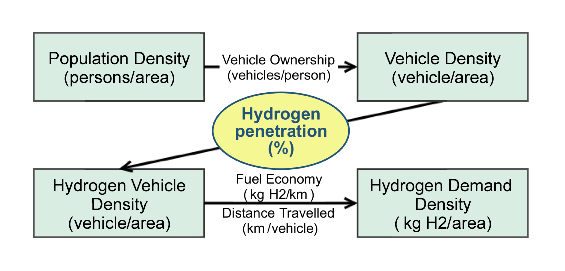
\includegraphics[width=0.75\textwidth]{FIG_11}
\caption{\label{fig:CommonMethodDemand}Common method for hydrogen demand estimation}
\end{figure}

\citet{agnolucci2013designing} noted that the adoption of hydrogen is expected to follow a logistic, S-shaped curve, which is similar to that observed in most of the new technologies. Three parameters describing the logistic substitution curve are the saturation point, ``anchoring" date (the start of the transition), and transition duration. \citet{almansoori2009design} explained the S-shaped curve: during the introductory stage of a hydrogen economy, the demand would be limited to a fleet of vehicles with a fixed daily route and regular refueling intervals at specific locations, e.g., buses. When the manufacturing cost of the FCEVs becomes affordable, and constraints, such as onboard storage, are overcome, the demand trajectory might sharply increase. Eventually, as the market arrives at a state of saturation, the demand trajectory will level off. Although several authors adopted the logistic substitution curve, it was usually based on subjective assumptions, which means that it was assumed outside of any mathematical model.

\citet{melendez2008regional} proposed a framework for examining whether a particular market can potentially transition to hydrogen-based mobility by evaluating the socio-economic factors. As described in Fig. \ref{fig:ApproachHydrogenPenetration}, nine key attributes that affect hydrogen penetration into the consumer market are identified. By mapping the value of these socio-economic factors at the local level, an idea of the geographical and temporal evolution of hydrogen demand within a particular national context \citep{agnolucci2013designing} can be acquired. Each geographic area is scored according to each attribute; thereafter, these scores are added to obtain the final score. This final score identifies areas where hydrogen demand is presumed to be promising. Only two studies \citep{dayhim2014planning,moreno2017towards} that consider the socio-economic analysis are reported in the reference papers.

The third method of linking the energy system model with an HSCN model mainly refers to a MARKAL/TIMES model as mentioned in section \ref{sec:searchliter}. One of the fundamental characteristics of a MARKAL/TIMES model is that both supply and demand  are integrated; one automatically responds as the other changes. Considering this feature, it is possible to achieve a hydrogen demand profile by feeding MARKAL/TIMES model with a techno-economic specification. The method of linking the energy system model with an HSCN model is schematized in Fig. \ref{fig:ApproachHydrogenPenetration}. 

\begin{figure}[!htbp]
\centering
\includegraphics[width=1\textwidth]{FIG_12}
\caption{\label{fig:ApproachHydrogenPenetration}Three approaches to determine hydrogen penetration}
\end{figure}

\citet{agnolucci2013designing} noted that apart from studies that use energy system models, most studies dealing with the modeling of an HSC assumed an exogenous trajectory of hydrogen demand. Moreover, several studies do not consider the evolution of a system over time. Only one study implemented a comparatively comprehensive estimation of the hydrogen demand that considered logistic substitution curve, socio-economic analysis, and energy system model \citep{agnolucci2013importance}. The estimation process is schematized in Fig. \ref{fig:DemandForecastingAgnolucci}. Firstly, a hydrogen demand scenario (the HyWay European Hydrogen) \citep{EU2008hyways} defined two of the parameters that describe a logistic substitution curve: saturation point and transition duration. Thereafter, the authors adopted an energy system model (named UK MARKAL) to indicate when hydrogen may be introduced to make the transition consistent with the broader analysis of cost-optimal decarbonization trajectories (known as ``anchoring'' date). Afterwards, a socio-economic analysis was conducted to identify the spatial distribution of hydrogen demand, specifically, the transition order of subregions. In this way, a set of several diffusion curves was assigned to the geographical area. By stacking these curves and considering a typically faster diffusion rate in regions that are slow to adopt, a profile of the hydrogen penetration was purchased.

\begin{figure}[!htbp]
\centering
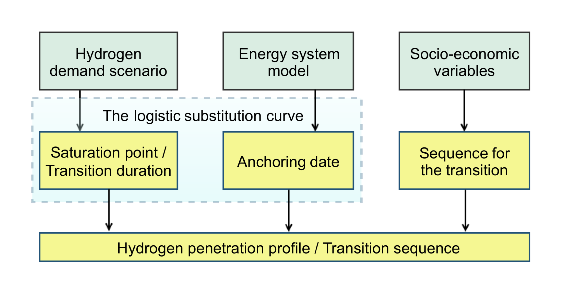
\includegraphics[width=0.65\textwidth]{FIG_13}
\caption{\label{fig:DemandForecastingAgnolucci}Demand forecasting process in the work of \citet{agnolucci2013importance}}
\end{figure}

\section{General conclusions and research directions}
\label{sec:synthesis}

This paper presents an overview of the research development regarding the use of optimization methods for the hydrogen supply chain network design. Separate sections are dedicated to analyze and classify the selected papers according to system analysis, decision variables, performance measures, uncertainties, and solution approaches in order to clearly identify the gaps in the literature and determine research opportunities and future directions. It is evident in the various tables presented throughout the review that several research directions still require intensive research.

This study demonstrates that the HSCND models currently focus on the use of domestic feedstocks for hydrogen production. International trades of hydrogen, however, may also provide win-win opportunities to both exporting and importing countries. Inevitably, long-distance transportation involved in international hydrogen trading as well as in multi-national or cross-regional financing activities may become another problem. Two studies considered the import of feedstock from other countries \citep{almansoori2012design,almansoori2009design}. \citet{moreno2017towards} took into account the possibility of the international importation of liquid hydrogen. However, it has not led to any comprehensive study that encompasses all the echelons of an international HSCN. Accordingly, further research is necessary on this aspect. 

The intertemporal integration planning, which incorporates various activities over strategic, tactical, and operational planning horizons, has been overlooked in the HSCND models. It is suggested that the location/routing problem is the most relevant subject for future studies of the HSCND because the major trade-off in it is between the transportation cost, and capital and production costs of manufacturing facilities. Moreover, the strategic decisions that would be made in isolation might be different from those that would be made by taking into account the routing problem. This means that intertemporal integration planning could aid researchers to gain further insight on the HSCND. 

Concerning performance measures, it is shown that a majority of the studies reported in the reference papers are cost-oriented. The minimal share of the multi-objective models in the HSCND models indicate that there is an existing gap in the literature. Apart from environmental impact and safety, other measures could be introduced into the HSCND models. For example, as a renewable alternative, the efficiency of energy use in the HSCN is also an important indicator. Another aspect of evaluating the SCN performance is in terms of the social benefit it provides. Similar to the biomass supply chain network \citep{yue2014biomass}, the most critical perspective in the social dimension for the HSCN may be the impact on employment, which can be measured by the number of accrued local jobs (full-time equivalent for a year) in a regional economy.

Another aspect that requires more attention is the uncertainty. Although half of the studies reported in the reference papers took this into account, the source of uncertainty is limited to hydrogen demand (strategic level). Other sources, such as government incentives and policies, technology evolution, capital cost, as well as the operational uncertainties are ignored in the HSCND models. Concerning uncertainty types and modeling approaches, random uncertainties are evaluated using scenario analysis and stochastic programming in most related studies. Accordingly, the inclusion of epistemic uncertainty, deep uncertainty, and corresponding modeling approaches, particularly robust optimization, is a future direction for researchers who are interested in uncertainty problems. 

A hydrogen supply system is not isolated; it is an integral part of the entire energy system. A broader perspective may offer more suitable solutions. Its integration with other supply chains is an important research direction. The critical factor for such an integration is to identify the appropriate ``insertion points'' through which the two supply chains are connected \citep{yue2014biomass}. For the HSCN, such ``insertion points'' are not difficult to identified. The several studies presented in the reference papers could serve as good examples. In the work of \citet{cho2016optimization,parker2010waste}, and \citet{woo2016optimization}, the modeling and optimization of an HSCN is conducted with a biomass supply chain. \citet{kim2017integrated} discussed the integration of an HSCN with a wind power generation system. In the work of \citet{hwangbo2017mathematical}, the HSCN was associated with a utility supply network, and the SMR process was used as a linkage (insertion point) between the two networks. Furthermore, \citet{bique2018integration} developed an MILP model for the integration of hydrogen and CO$_{2}$ supply chains, and the production of methanol links the two networks together. Beyond that, other feedstocks (e.g., electricity from solar energy or nuclear energy), byproducts (e.g., oxygen from electrolysis), and final products (hydrogen for other uses, e.g., industry or ``Power to Gas'' project \citep{welder2018spatio}) could serve as ``insertion points'' to conduct more integrations. Therefore, there remain several areas for enhancing the development of new models and thereby aid in the decision-making process in an integrated HSCN planning.


\section*{Acknowledgement}
This work is financially supported by a program of the China Scholarship Council for Ph.D. Scholarship No. 201604490065.

\section*{References}
\bibliography{shortbibfile}

\section*{Supplementary material}
Supplementary material can be found in the submission files, with the name of \\ \textit{SupplementaryMaterial.xlsx}.


\end{document}